%!Mode:: "TeX:UTF-8"
\documentclass[a4paper,11pt,UTF8]{ctexart}

\usepackage{indentfirst} %缩进
\usepackage{xeCJK}    %使用系统字体
\usepackage{fancyhdr} %自定义页眉页脚
\pagestyle{empty}                   %不设置页眉页脚
\usepackage{amsmath, amsthm, amssymb, amsfonts} %数学公式
\usepackage[a4paper,left=3cm,right=3cm,top=3cm,bottom=3cm]{geometry}
%\usepackage[tmargin=1in,bmargin=1in,lmargin=1.25in,rmargin=1.25in]{geometry}.
\usepackage{booktabs} %插入表格
\usepackage[section]{placeins} %避免浮动
\usepackage{listings} %插入代码
\usepackage{ctex}     %中文宏包
\usepackage[svgnames, table]{xcolor} %彩色表格
\usepackage{algorithm}          %伪代码
\usepackage{algorithmicx}
\usepackage{algpseudocode}
\usepackage{algorithm,algpseudocode,float}
\usepackage{lipsum}
\usepackage{enumitem}           %调整列举环境
\usepackage{url}
\usepackage{fontspec,xunicode}
\defaultfontfeatures{Mapping=tex-text} %如果没有它,会有一些 tex 特殊字符无法正常使用,比如连字符。

\usepackage{graphicx}
\graphicspath{{imgs/}}

%%%%%%%%%%%%%%%%%%%%%%%%%%%%%%%%%%%%%%%%%%%%%%%%%%%%%%%%%%%%%%%%
% 缩进及行间距
%%%%%%%%%%%%%%%%%%%%%%%%%%%%%%%%%%%%%%%%%%%%%%%%%%%%%%%%%%%%%%%%
\setlength{\parindent}{22pt} %重新定义缩进长度
\setlength{\baselineskip}{20pt}  %定义行间距
%\renewcommand{\baselinestretch}{1.1} %定义行间距

%%%%%%%%%%%%%%%%%%%%%%%%%%%%%%%%%%%%%%%%%%%%%%%%%%%%%%%%%%%%%%%%
% 列表设置
%%%%%%%%%%%%%%%%%%%%%%%%%%%%%%%%%%%%%%%%%%%%%%%%%%%%%%%%%%%%%%%%
\setenumerate{fullwidth,itemindent=\parindent,listparindent=\parindent,itemsep=0ex,partopsep=0pt,parsep=0ex}
\setenumerate[2]{label=\alph*),leftmargin=1.5em}  %二级item设置
\setitemize{itemindent=38pt,leftmargin=0pt,itemsep=-0.4ex,listparindent=26pt,partopsep=0pt,parsep=0.5ex,topsep=-0.25ex}
\setdescription{itemindent=38pt,leftmargin=0pt,itemsep=-0.4ex,listparindent=26pt,partopsep=0pt,parsep=0.5ex,topsep=-0.25ex}

%%%%%%%%%%%%%%%%%%%%%%%%%%%%%%%%%%%%%%%%%%%%%%%%%%%%%%%%%%%%%%%%
% 图的标题行间距设置
%%%%%%%%%%%%%%%%%%%%%%%%%%%%%%%%%%%%%%%%%%%%%%%%%%%%%%%%%%%%%%%%
\newcommand{\bottomcaption}{%
\setlength{\abovecaptionskip}{6pt}%
\setlength{\belowcaptionskip}{6pt}%
\caption}


%%%%%%%%%%%%%%%%%%%%%%%%%%%%%%%%%%%%%%%%%%%%%%%%%%%%%%%%%%%%%%%%
% 字体定义
%%%%%%%%%%%%%%%%%%%%%%%%%%%%%%%%%%%%%%%%%%%%%%%%%%%%%%%%%%%%%%%%
\setmainfont{Times New Roman}  %默认英文字体.serif是有衬线字体sans serif无衬线字体
\setmonofont{Consolas}
\setCJKmainfont[ItalicFont={楷体}, BoldFont={黑体}]{宋体}%衬线字体 缺省中文字体为
\setCJKsansfont{黑体}
\punctstyle{hangmobanjiao}
%-----------------------xeCJK下设置中文字体------------------------------%
\setCJKfamilyfont{song}{SimSun}                             %宋体 song
\newcommand{\song}{\CJKfamily{song}}
\setCJKfamilyfont{fs}{FangSong}                      %仿宋  fs
\newcommand{\fs}{\CJKfamily{fs}}
\setCJKfamilyfont{ktgb}{KaiTi}                      %楷体2312 ktgb
\newcommand{\ktgb}{\CJKfamily{ktgb}}
\setCJKfamilyfont{yh}{Microsoft YaHei}                    %微软雅黑 yh
\newcommand{\yh}{\CJKfamily{yh}}
\setCJKfamilyfont{hei}{SimHei}                              %黑体  hei
\newcommand{\hei}{\CJKfamily{hei}}
\setCJKfamilyfont{hwxk}{STXingkai}                                %华文行楷  hwxk
\newcommand{\hwxk}{\CJKfamily{hwxk}}
%------------------------------设置字体大小------------------------%
\newcommand{\shiyanbaogao}{\fontsize{36pt}{\baselineskip}\selectfont}
\newcommand{\chuhao}{\fontsize{42pt}{\baselineskip}\selectfont}     %初号
\newcommand{\xiaochuhao}{\fontsize{36pt}{\baselineskip}\selectfont} %小初号
\newcommand{\yihao}{\fontsize{28pt}{\baselineskip}\selectfont}      %一号
\newcommand{\erhao}{\fontsize{21pt}{\baselineskip}\selectfont}      %二号
\newcommand{\xiaoerhao}{\fontsize{18pt}{\baselineskip}\selectfont}  %小二号
\newcommand{\sanhao}{\fontsize{15.75pt}{\baselineskip}\selectfont}  %三号
\newcommand{\sihao}{\fontsize{14pt}{\baselineskip}\selectfont}       %四号
\newcommand{\xiaosihao}{\fontsize{12pt}{\baselineskip}\selectfont}  %小四号
\newcommand{\wuhao}{\fontsize{10.5pt}{\baselineskip}\selectfont}    %五号
\newcommand{\xiaowuhao}{\fontsize{9pt}{\baselineskip}\selectfont}   %小五号
\newcommand{\liuhao}{\fontsize{7.875pt}{\baselineskip}\selectfont}  %六号
\newcommand{\qihao}{\fontsize{5.25pt}{\baselineskip}\selectfont}    %七号

%%%%%%%%%%%%%%%%%%%%%%%%%%%%%%%%%%%%%%%%%%%%%%%%%%%%%%%%%%%%%%%%
% 图题字体大小相同
%%%%%%%%%%%%%%%%%%%%%%%%%%%%%%%%%%%%%%%%%%%%%%%%%%%%%%%%%%%%%%%%
\usepackage{caption}
\captionsetup{font={footnotesize}}   % footnotesize = 9pt
\captionsetup[lstlisting]{font={footnotesize}}

%%%%%%%%%%%%%%%%%%%%%%%%%%%%%%%%%%%%%%%%%%%%%%%%%%%%%%%%%%%%%%%%
% 重定义枚举编号为 1),2)...
%%%%%%%%%%%%%%%%%%%%%%%%%%%%%%%%%%%%%%%%%%%%%%%%%%%%%%%%%%%%%%%%
\renewcommand{\labelenumi}{\theenumi)}

%%%%%%%%%%%%%%%%%%%%%%%%%%%%%%%%%%%%%%%%%%%%%%%%%%%%%%%%%%%%%%%%
% 标题名称中文化
%%%%%%%%%%%%%%%%%%%%%%%%%%%%%%%%%%%%%%%%%%%%%%%%%%%%%%%%%%%%%%%%
\renewcommand\figurename{\hei 图}
\renewcommand\tablename{\hei 表}
\renewcommand\lstlistingname{\hei 代码}
\renewcommand{\algorithmicrequire}{\textbf{输入:}}
\renewcommand{\algorithmicensure}{\textbf{输出:}}
\newtheorem{define}{定义}

%%%%%%%%%%%%%%%%%%%%%%%%%%%%%%%%%%%%%%%%%%%%%%%%%%%%%%%%%%%%%%%%
% 代码设置
%%%%%%%%%%%%%%%%%%%%%%%%%%%%%%%%%%%%%%%%%%%%%%%%%%%%%%%%%%%%%%%%
\lstset{
 columns=fixed,
 numbers=left,                                        % 在左侧显示行号
 numberstyle=\tiny\color{gray},                       % 设定行号格式
 frame=single,                                        % 单线背景边框
 breaklines=true,                                     % 设定LaTeX对过长的代码行进行自动换行
 keywordstyle=\color[RGB]{40,40,255},                 % 设定关键字颜色
 numberstyle=\footnotesize\color{darkgray},
 commentstyle=\it\color[RGB]{0,96,96},                % 设置代码注释的格式
 stringstyle=\rmfamily\slshape\color[RGB]{128,0,0},   % 设置字符串格式
 showstringspaces=false,                              % 不显示字符串中的空格
 language=java,                                        % 设置语言
 basicstyle=\linespread{1.0}\xiaowuhao\ttfamily,                      % 字体字号
 %lineskip=10pt,
 %baselinestretch=1,
}

%%%%%%%%%%%%%%%%%%%%%%%%%%%%%%%%%%%%%%%%%%%%%%%%%%%%%%%%%%%%%%%%
% 伪代码分页
%%%%%%%%%%%%%%%%%%%%%%%%%%%%%%%%%%%%%%%%%%%%%%%%%%%%%%%%%%%%%%%%
\makeatletter
\renewcommand{\ALG@name}{算法}
\newenvironment{breakablealgorithm}
  {% \begin{breakablealgorithm}
   \begin{center}
     \refstepcounter{algorithm}% New algorithm
     \hrule height.8pt depth0pt \kern2pt% \@fs@pre for \@fs@ruled
     \renewcommand{\caption}[2][\relax]{% Make a new \caption
       {\raggedright\textbf{\ALG@name~\thealgorithm} ##2\par}%
       \ifx\relax##1\relax % #1 is \relax
         \addcontentsline{loa}{algorithm}{\protect\numberline{\thealgorithm}##2}%
       \else % #1 is not \relax
         \addcontentsline{loa}{algorithm}{\protect\numberline{\thealgorithm}##1}%
       \fi
       \kern2pt\hrule\kern2pt
     }
  }{% \end{breakablealgorithm}
     \kern2pt\hrule\relax% \@fs@post for \@fs@ruled
   \end{center}
  }
\makeatother

% =============================================
% Part 1 Edit the info
% =============================================

\newcommand{\major}{物理学院}
\newcommand{\name}{黄阅迅,李秋阳}
\newcommand{\stuid}{PB18020631,PB18020567}
\newcommand{\group}{20}
\newcommand{\newdate}{\today}


\newcommand{\course}{电子线路实验(1)}
\newcommand{\newtitle}{二极管的基本应用}

% =============================================
% Part 1 Main document
% =============================================
\begin{document}
\thispagestyle{empty}
\begin{figure}[h]
  \begin{minipage}{0.6\linewidth}
    \centerline{
\includegraphics[width=\linewidth]{logo.png}}
  \end{minipage}
  \hfill
  \begin{minipage}{.4\linewidth}
    \raggedleft
    \begin{tabular*}{.8\linewidth}{ll}
      学院: & \underline\major   \\
      姓名: & \underline\name    \\
      学号: & \underline\stuid   \\
      组号:  & \underline\group   \\
      日期: & \underline\newdate \\
    \end{tabular*}
  \end{minipage}
\end{figure}

\begin{table}[!htbp]
  \centering
  \begin{tabular*}{\linewidth}{llllll}
    课程名称:  \underline\course   \qquad\qquad 实验题目:  \underline\newtitle  
  \end{tabular*}
\end{table}

% =============================================
% Part 2 Main document
% =============================================

\section{实验目的}

参看预习报告。

\section{实验原理}

部分内容参看预习报告。以下为补充内容。

\subsection{整流滤波电路}
如图 \ref{fig:SVCsim}为最简单的整流电路,其中包含一个二极管与负载电阻$R_L$,当正板周期时,二极管导通,负半周时,二极管截止。
由此达到整流目的,其输出波形如图右侧所示。
\begin{figure}[htbp]
  \centering
  \fbox{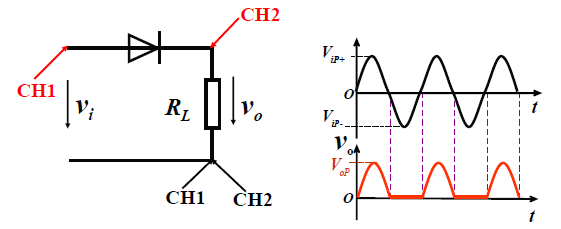
\includegraphics[width=0.5\linewidth]{SVCsim}}
  \caption{整流电路电路与波形示意图}
  \label{fig:SVCsim}
  \end{figure}
则理论上可以计算出输出电压的平均值为
\begin{equation}
  \bar{V}_0=\frac{1}{T}\int_0^Tv_0(t)dt=\frac{V_p}{\pi}\approx0.318V_p
\label{eqa:avgV_SVC}
\end{equation}
当并联电容时,电容的阻抗随频率增大而减小,因此可以起到一定的滤高频波的作用,其电路图及波形如图 \ref{fig:SVCcom}所示。
\begin{figure}[htbp]
  \centering
  \fbox{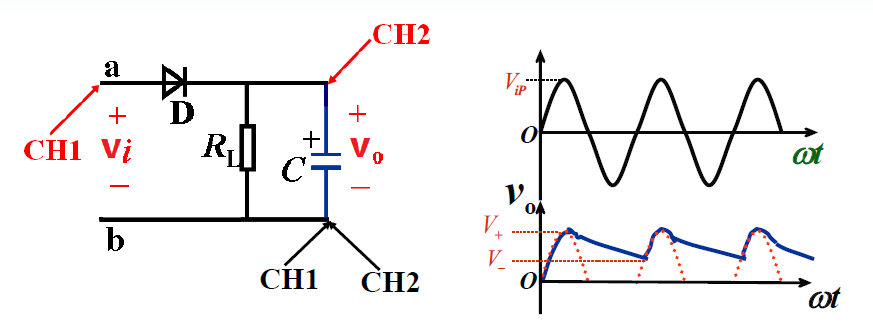
\includegraphics[width=0.5\linewidth]{SVCcom}}
  \caption{整流滤波电路电路与波形示意图}
  \label{fig:SVCcom}
  \end{figure}

\subsection{钳位电路}
其电路与波形如图 \ref{fig:clamper}所示。二极管作理想处理,当输入正弦波时,当$V_i$上升到$E$时,二极管D导通,$V_o$就不可能再上升,被钳位
在这一电平上。$V_i$继续上升,多余的电压被充到电容C上,由于二极管正向导通电阻很小,充电很快,电容电压可充到$V_p-E$。
当$V_i$电压从峰值下降时,二极管截止,输出电压$V_o$为电容上电压和$V_i$的代数和。整个波形被压下$V_p-E$伏,顶端被钳制在E上,均值即在E(注意符号)附近。
但实际上二极管有压降,实际分析时需要考虑二极管压降。
\begin{figure}[htbp]
  \centering
  \fbox{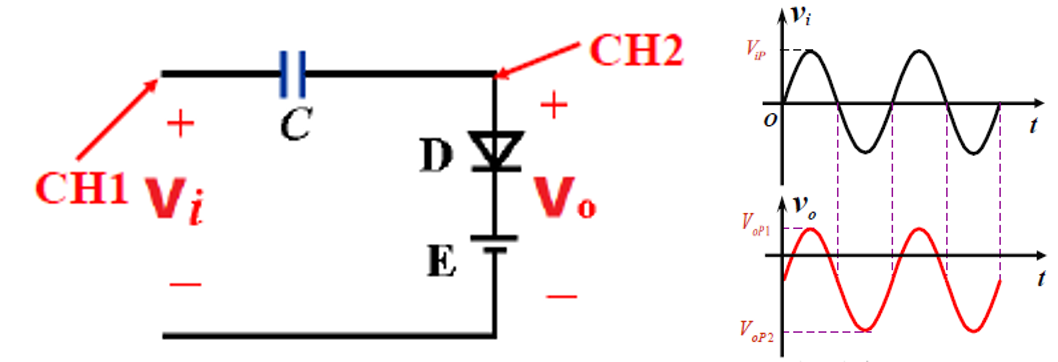
\includegraphics[width=0.5\linewidth]{clamper}}
  \caption{钳位电路电路电路与波形示意图}
  \label{fig:clamper}
  \end{figure}

\subsection{限幅电路}
限幅电路,又称削波电路,是用来限制输出信号电压范围的电路,仅有上门限的称为上限幅
电路,仅有下门限的称为下限幅电路,具有上下门限的限幅电路,称为双向限幅电路。其工作原理与整流电路相近,由于恒压源的存在,使得当输入电压加上恒压源一旦超出了二
极管的导通范围,就会截止,因此具有限制幅度的功能。其电路与输出波形如图 \ref{fig:limiter}所示。二极管作理想处理,当输入正弦波时,当
\begin{figure}[htbp]
  \centering
  \fbox{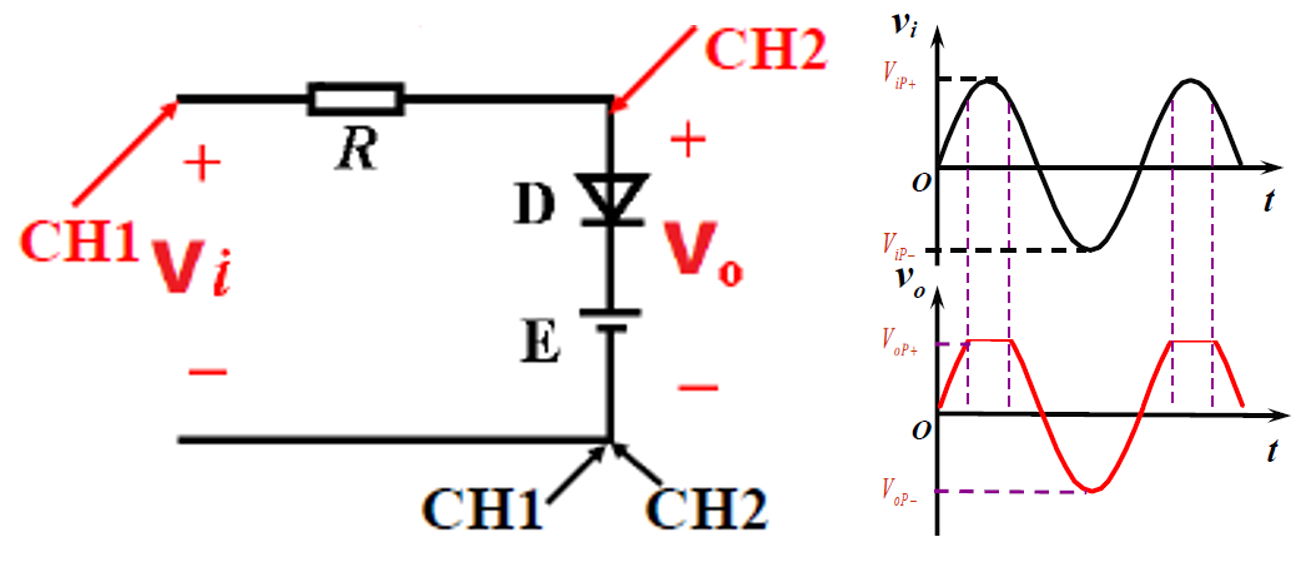
\includegraphics[width=0.5\linewidth]{limiter}}
  \caption{限幅电路电路与波形示意图}
  \label{fig:limiter}
  \end{figure}

\subsection{稳压电路}
其电路图如图 \ref{fig:stabler}所示。当负载$R_L$一定时,如果$V_i$增大,则$V_z$增大,由于稳压二极管动态电阻很小,干路的电流基本上被其捕获,因此$R_1$上的压降增大,最终$V_o$几乎不变。
当$R_L$减小时,则其干路路电流增大,因此干路压降增大,则$V_z$分压减小,最终$V_o$基本不变。
\begin{figure}[htbp]
  \centering
  \fbox{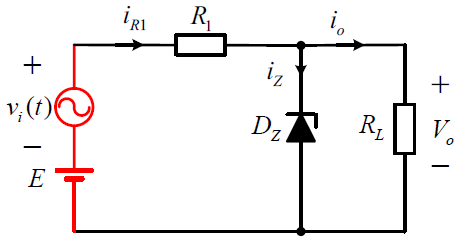
\includegraphics[width=0.5\linewidth]{stabler}}
  \caption{限幅电路电路与波形示意图}
  \label{fig:stabler}
  \end{figure}


\section{实验内容与步骤}
\subsection{实验内容}
	blablabla
\subsection{实验步骤}
	blablabla

\section{实验数据处理与分析}
\subsection{实验内容1}
	blablabla
\subsection{误差分析1}
	blablabla

\section{实验总结}
blablabla
\section{实验思考题}
\subsection{问题一}
二极管,对直流量,它相当于一个电压源,而对交流量,它等效成一个小电阻,这句话对吗?稳压管有何特性?

\textbf{答:}这句话需要添加更多的修饰条件,不完全正确。对于直流量,二极管导通时,可以采用恒压降模型,认为其管压降恒定,因此
可以近似成一个电压源,对于硅管,一般是$0.7V$,对于锗管,一般是$0.2V$。但电压很大时,应采用折线模型修正,看作一个有内阻的电压源。

对于交流分量,需要在小信号分析的前提下,采用小信号模型,其可以看作是一个小电阻,在只考虑交流量的情况下,有$r_d\approx\frac{V_T}{I_D}$,$V_T$为电压当量,$I_D$为Q点二极管电流。因此要求为小信号条件下,才可以看作为
小电阻。

稳压二极管,又称为齐纳二极管,这种管子杂质浓度很高,空间电荷区内的电荷密度很大,因而区域窄,容易形成强电场。当反向击穿时,反向电压波动不大即有较大的电流变化。但不能超过最大工作电流,否则进入反向特性转弯段,稳压特性消失,可能被烧毁。
\subsection{问题二}
说明稳压管并联稳压电路的稳压原理。

\textbf{答:}该电路的核心在于稳压管与并联。稳压管工作于反向击穿状态下时,其工作电压随电流变化很小,因此起到稳压作用。

而稳压管由于电压随电流变化很小,因此其动态电阻$r_z$非常小,因此将外界扰动导致的干路电流变化看作小信号。其在并联电路的作用下,由于稳压管动态电阻很小,小信号波动基本上会被
稳压管全部拾取,而稳压管电压随电流变化很小,因此稳压管在拾取了变化量后电压几乎维持不变,因此与之并联的输出电压也几乎不发生变化。

具体地说:当负载$R_L$一定时,如果$V_i$增大,则$V_z$增大,由于稳压二极管动态电阻很小,干路的电流基本上被其捕获,因此$R_1$上的压降增大,最终$V_o$几乎不变。
当$R_L$减小时,则干路路电流增大,因此干路压降增大,则$V_z$分压减小,最终$V_o$基本不变。反之亦然。

\newpage
\begin{appendix}

\section{代码示例}

\begin{lstlisting}[caption={一段C代码},captionpos=b]
#include <stdio.h>
int main (int argc, char *argv[]){
  printf("Hello world!");
}
\end{lstlisting}

\section{表格示例}
表 \ref{tab:tab1}与表 \ref{tab:tab2}展示了表格示例
\begin{table}[!h!tbp]
\caption{一个简单的表格}\label{tab:tab1}
  \centering
  \begin{tabular}{|l|c|c|}
	\hline
	功能          &WEB         &APP         \\ \hline
	注册          &$\surd$     &$\surd$     \\ \hline
	登录          &$\surd$     &$\surd$     \\ \hline
	推送          &$\times$    &$\surd$     \\ \hline
\end{tabular}
\end{table}

\begin{table}[!h!tbp]
\caption{自定义表格}\label{tab:tab2}
  \centering
\begin{tabular*}{0.75\textwidth}{@{\extracolsep{\fill}}lcc}
    \toprule
    功能          &WEB         &APP         \\
    \midrule
    注册          &$\surd$     &$\surd$     \\
    登录          &$\surd$     &$\surd$     \\
    推送          &$\times$    &$\surd$     \\
    \bottomrule
\end{tabular*}
\end{table}


\section{图片示例}
图 \ref{fig:logo}展示了一个图片示例。
\begin{figure}[htbp]
\centering
\fbox{
\includegraphics[width=0.5\linewidth]{logo}}
\caption{blablabla}
\label{fig:logo}
\end{figure}

\section{公式示例}
式 (\ref{eqa:01})展示了一个公式的例子。
\begin{equation}
S_n = \frac{X_1 + X_2 + \cdots + X_n}{n}
      = \frac{1}{n}\sum_{i}^{n} X_i
\label{eqa:01}
\end{equation}




\end{appendix}

\end{document}
